% \chapter{Simulação e Resultados}
\chapter{Resultados e Discussão}

Para analisar as capacidades do modelo proposto, foram realizados três experimentos. Os dois primeiros experimentos foram implementados utilizando o design $2^k$ fatorial \cite{jain1990art}. Esse tipo de design consiste em variar $k$ fatores em 2 níveis diferentes, -1 e 1, que são extremos opostos. Por exemplo, em uma pesquisa ligada a um processador, um fator pode ser o número de núcleos, e seus níveis serem 1 núcleo e 8 núcleos. Portanto, o fator é uma variável livre, que é utilizada para analisar a variação de uma variável dependente qualquer. Os fatores e as variáveis livres utilizadas estão nas tabelas \ref{table:experiments_factors} e \ref{table:experiments_variables}, respectivamente. A análise do impacto dos fatores foi realizada utilizando a equação de regressão não linear do design $2^k$ fatorial. 
%O código implementado para essa análise está disponível no anexo [NÚMERO].

\begin{table}[h!]
    \begin{center}
        \caption{ Fatores utilizados nos experimentos. }
        \label{table:experiments_factors}
        \begin{tabular}{|c|c|c|c|}
        \hline
        \textbf{Fatores} & \textbf{Sigla} & \textbf{Nível -1} & \textbf{Nível 1} \\
        \hline
        Porcentagem de Percepções Inválidas & PPI & 5\% & 95\%  \\
        \hline
        Tempo Médio Gasto Pelo Autoplanejamento & TMA & 1/2 CR & 64 CR \\
        \hline
        Tempo Médio Gasto em um Ciclo de Raciocínio & TMC & 01 CR & 32 CR \\
        \hline
        Número de Percepções Recebidas por Ciclo & NPC & 01 & 16 \\
        \hline
    \end{tabular}{}
    \end{center}
\end{table}{}

\begin{table}[h!]
    \begin{center}
        \caption{ Variáveis dependentes analisadas nos experimentos. }
        \label{table:experiments_variables}
        \begin{tabularx}{\textwidth}{ |Y|Y| }
            \hline
            \textbf{Variáveis} & \textbf{Justificativa} \\
            \hline
            Tempo Virtual Decorrido & Medir desempenho geral do modelo \\
            \hline
            Planos Criados & Avaliar potencial do modelo de inserir aprendizado em arquiteturas que não o possuem \\
            \hline
            Percepções Processadas & Analisar a capacidade do modelo de ganhar desempenho ao longo do tempo\\
            \hline
        \end{tabularx}{}
    \end{center}{}
\end{table}

As simulações consistem na execução do modelo proposto, que foi implementado em Python, submetido a um grande volume de percepções. O agente utilizado na simulação segue os exemplos apresentados no capítulo 4 (robô embrulhador).
Uma simulação possui 5000 ciclos, sendo que cada ciclo pode possuir uma ou várias percepções. Essas percepções podem ser válidas (pertencentes ao contexto do agente) ou inválidas (não pertencentes ao contexto do agente), sendo que a proporção entre o tipo de percepções é definido pela PPI. As percepções são produzidas aleatoriamente por um gerador de percepções. As percepções válidas são geradas sorteando percepções que pertencem ao contexto do agente, e as percepções inválidas são geradas utilizando o pacote \texttt{RandomWords} \cite{pipRandomWords}. Cada ciclo da simulação segue os seguintes passos:

\begin{enumerate}
    \item Gerar as percepções da simulação;
    \item Iterar sobre cada um dos ciclos, passando as percepções para o modelo implementado;
    \item Salvar os resultados, o agente final (com novos planos gerados pelo módulo de planejamento automatizado) e as percepções de cada ciclo em arquivos CSV.
\end{enumerate}

\begin{figure}[h!]
    \centering
    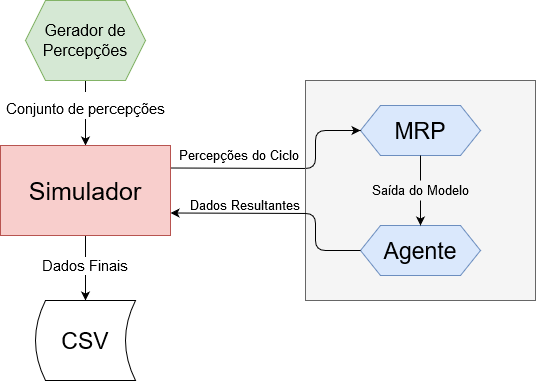
\includegraphics[width=0.8\textwidth]{Images/diagrama-simulacao.png}
    \caption{Diagrama da execução de uma iteração de cada experimento.}
    \label{fig:diagrama-simulacao}
\end{figure}

Além da configuração dos valores dos fatores, é possível configurar se um agente será recarregado (ou seja, se ele deve manter os planos gerados por uma simulação anterior) e se o simulador deve gerar novas percepções ou não, pulando a etapa 1 de cada ciclo.

Como é um experimento feito para uma arquitetura cognitiva genérica, vamos supor que o tempo de processamento que o agente gasta em cada ciclo de raciocínio é constante, e o tempo gasto pelo módulo de planejamento automatizado será calculado em função desse valor, ou seja, se o tempo do ciclo de raciocínio é o mesmo do planejamento automatizado, vamos dizer que o tempo do planejamento automatizado é 1 CR (ciclo de raciocínio).

\section{Experimento 1}

O objetivo do primeiro experimento é analisar a variação no tempo do ciclo de raciocínio e a quantidade de planos criados pelo módulo de planejamento automatizado, de acordo variações nos quatro fatores apresentados. Cada simulação foi repetida dez vezes, para que uma média pudesse ser obtida. Apesar do uso de repetições, não foi usada a metodologia do design $2^k r$ fatorial, que considera as possíveis falhas referente as repetições, pois o resíduo dos experimentos é extremamente baixo, da ordem de grandeza de $e^{-12}$.

\subsection{Resultados}

A média dos resultados de cada simulação estão apresentados na tabela \ref{table:experimento1.}. Os valor final do tempo virtual decorrido varia bastante, principalmente nas simulações com alto nível de percepções inválidas. Em dois momentos o tempo virtual foi 5000. Isso ocorreu pois nessas simulações o TMC é 1, o TMA é 0.5 e o NPC é 16. Portanto, ciclos de percepções válidas consumiam 1 unidade de tempo (4750). O bloco avaliados sempre permitia o processamento de 2 percepções inválidas (pois cada uma toma 0.5 unidades de tempo), e quase sempre há percepções inválidas disponíveis na fila pois entram 16 percepções inválidas por ciclo de percepções inválidas. Portanto, cada vez que o modelo processava percepções inválidas, ele consumia 1 unidade de tempo, e isso aconteceu 250 vezes (5\% de 5000).

\begin{table}[h!]
    \begin{center}
        \caption{ Resultados do experimento 1}
        \label{table:experimento1}
        \begin{tabular}{ |c|c|c|c|c|c|c| }
            \hline
            \textbf{Simulação} & \textbf{PPI} & \textbf{TMC} & \textbf{TMA} & \textbf{NPC} & \textbf{Tempo Virtual} & \textbf{Planos Criados}\\
            \hline
            1 & 5\% & 1 & 1/2 & 1 & 4874.6 & 250.8\\
            \hline
            2 & 5\% & 1 & 1/2 & 16 & 5000.0 & 502.0\\
            \hline
            3 & 5\% & 1 & 64 & 1 & 20806.7 & 250.9\\
            \hline
            4 & 5\% & 1 & 64 & 16 & 20813.0 & 251.0\\
            \hline
            5 & 5\% & 32 & 1/2 & 1 & 152093.5 & 251.0\\
            \hline
            6 & 5\% & 32 & 1/2 & 16 & 153437.3 & 2932.2\\
            \hline
            7 & 5\% & 32 & 64 & 1 & 168028.8 & 250.9\\
            \hline
            8 & 5\% & 32 & 64 & 16 & 168032.0 & 251.0\\
            \hline
            9 & 95\% & 1 & 1/2 & 1 & 3229.2 & 3541.6\\
            \hline
            10 & 95\% & 1 & 1/2 & 16 & 5000.00 & 9303.8\\
            \hline
            11 & 95\% & 1 & 64 & 1 & 228668.9 & 3550.3\\
            \hline
            12 & 95\% & 1 & 64 & 16 & 304300.4 & 4750.8\\
            \hline
            13 & 95\% & 32 & 1/2 & 1 & 48521.5 & 3539.0\\
            \hline
            14 & 95\% & 32 & 1/2 & 16 & 140683.3 & 4073.8\\
            \hline
            15 & 95\% & 32 & 64 & 1 & 273609.6 & 3550.3\\
            \hline
            16 & 95\% & 32 & 64 & 16 & 312032.0 & 4751.0\\
            \hline
        \end{tabular}{}
    \end{center}{}
\end{table}

O número de planos criados se agruparam em certos conjuntos de valores, de acordo com os níveis dos fatores. Como esperado, as simulações com menor porcentagem de percepções inválidas criaram menos planos, pois houveram menos anomalias, logo menos material para o módulo de planejamento automatizado trabalhar. O gráfico da figura \ref{fig:pc_occurrences} mostra a ocorrência dos resultados em certos valores aproximados.

\begin{figure}[h!]
    \centering
    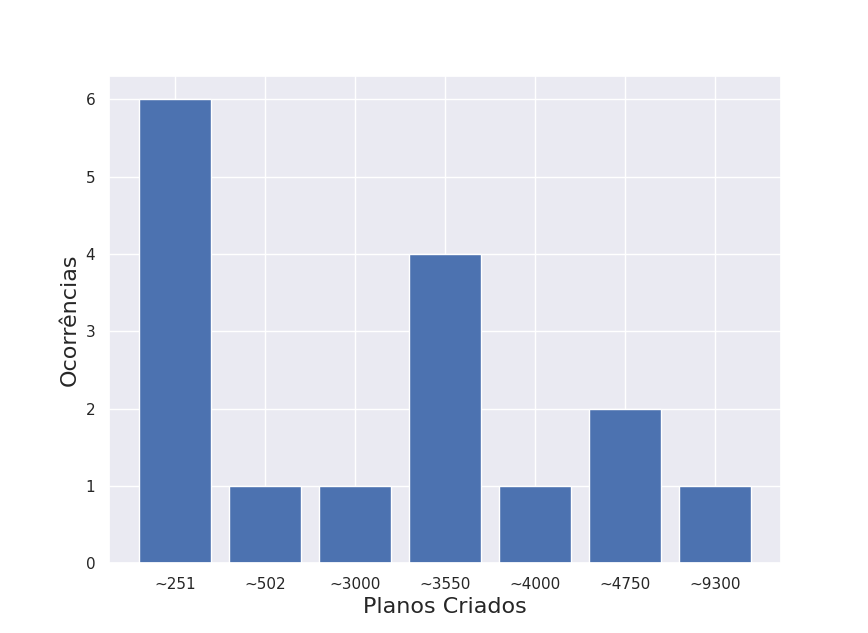
\includegraphics[width=0.8\textwidth]{Images/plans_created_occurrences.png}
    \caption{Recorrência do valor final de Planos Criados nas simulações realizadas.}
    \label{fig:pc_occurrences}
\end{figure}

\subsection{Análise de Fatores}

Conforme mostra a tabela \ref{tab:experimento1fatores}, na variável dependente de Tempo Virtual, os fatores TMC e TMA isolados tiveram uma alta porcentagem de impacto. Isso porque a contagem do tempo virtual acontecia em função justamente dos eventos de realizar planejamento automatizado e executar um ciclo de raciocínio. Portanto, a interferência nesses fatores influencia diretamente o resultado final. Além disso, a combinação dos fatores PPI + TMA teve um impacto bastante grande, de 24.13\%. Isoladamente, PPI e TMA possuem porcentagens altas (12.69 e 31.64, respectivamente), portanto era esperado que a sua
combinação também tivesse uma porcentagem alta. Entretanto, TMC possui 22.20 porcento de impacto, mas a combinação PPI + TMC possui apenas 4.16. Isso demonstra como uma combinação de alta taxa de percepções inválidas com um tempo de planejamento automatizado alto podem ser impactantes no resultado de um agente que executa o modelo.

\begin{table}
    \begin{center}
        \caption{Análise dos fatores do experimento 1}
        \label{tab:experimento1fatores}
        \begin{tabular}{ |c|c|c| }
            \hline
            \textbf{Fator} & \textbf{Efeito Tempo Virtual} & \textbf{Efeito Planos Criados}\\  
            \hline
            PPI & 12.69\% & 66.10\%\\
            \hline
            TMC & 22.20\% & 0.50\%\\
            \hline
            TMA & 31.64\% & 2.95\%\\
            \hline
            NPC & 1.44\% & 8.67\%\\
            \hline
            PPI + TMC & 4.16\% & 3.76\%\\
            \hline
            PPI + TMA & 24.13\% & 0.05\%\\
            \hline
            PPI + NPC & 1.39\% & 2.13\%\\
            \hline
            TMC + TMA & 0.55\% & 0.50\%\\
            \hline
            TMC + NPC & 0.10\% & 0.50\%\\
            \hline
            TMA + NPC & 0.01\% & 2.99\%\\
            \hline
            PPI + TMC + TMA & 0.53\% & 3.76\%\\
            \hline
            PPI + TMC + NPC & 0.09\% & 3.75\%\\
            \hline
            PPI + TMA + NPC & 0.02\% & 0.06\%\\
            \hline
            TMC + TMA + NPC & 0.54\% & 0.50\%\\
            \hline
            PPI + TMC + TMA + NPC & 0.52\% & 3.76\%\\
            \hline
        \end{tabular}{}
    \end{center}{}
\end{table}


Na variável dependente Planos Criados, a fator que mais impactou o resultado foi o PPI. Isso era o esperado, pois quanto mais percepções inválidas o modelo recebe, mais planos podem ser criados. Os outros fatores tiveram impactos bem mais baixos. O NPC teve 8.67\% de influência pois simulações com mais percepções inválidas por ciclo preenchem a fila ponderada mais rápido, sempre tendo combustível para alimentar o bloco de planejamento automatizado.

%%%%%%%%%%%%%%%%%%%%%%%%%%%%%%%%%%%%%%%%%%%%%%%%%%%%%%%%%%%%%%%%%%%%

\section{Simulação 2}

A segunda simulação foi realizada para analisar o ganho de performance de um agente ao aplicar os planos criados com o bloco de autoplanejamento. Esse segundo experimento segue os moldes do primeiro, porém foi realizado apenas uma iteração para cada configuração de fatores, e após ser realizado uma simulação com uma dada configuração, foi realizada uma nova simulação com os mesmos fatores, mas usando o agente resultante da primeira. Assim, os planos criados pelo agente foram reaproveitados.

Essa simulação pode ter sua configuração de fatores separadas em dois grupos: (I) o tempo de processamento de um ciclo de raciocínio é menor do que o tempo do autopĺanejamento; (II) o tempo do autoplanejamento é menor que o tempo de processamento de um ciclo de raciocínio. Essa separação pode ser feita pois quanto mais planos criados temos, menos percepções inválidas serão recebidas pelo agente. Portanto, se o tempo de processamento de um ciclo for maior que o de autoplanejamento, o tempo virtual gasto total usando um agente que já aprendeu vários planos será maior. Isso é um \textit{trade off} pois agora essas novas
percepções (que eram antes anomalias) estão efetivamente sendo utilizadas pelo agente.

\subsection{Resultados}

Os resultados estão separados em tabelas por variável dependente e por grupo, como descrito anteriormente. As tabelas contém o índice da simulação, os níveis dos fatores, os resultados da primeira e da segunda iteração (R1 e R2, respectivamente) e a relação percentual entre os resultados, ou seja, a proporção de R2 em relação a R1, obtido através do cálculo $(R2 * 100) / R1$.

Em todas as tabelas, podem ser observadas um menor efeito na relação percentual nas simulações que utilizaram o nível $-1$ do fator PPI (5\% de percepções inválidas). Isso se dá ao fato do menor impacto do modelo em ambientes de baixo volume de percepções inválidas, uma vez que o modelo apenas age quando há percepções inválidas na fila ponderada.

Na tabela \ref{table:vtaltv1}, a média da relação percentual foi de 75.26\%, se destacando a simulação 5 com uma relação percentual de 4.77\%. Com o tempo de autoplanejamento alto, tempo de processamento de um ciclo de raciocínio baixo e apenas uma percepção por ciclo, é notável o ganho de desempenho. Um comportamento similar (porém invertido) pode ser observado na tabela \ref{table:vtaltv2}, cuja média da relação percentual foi de 136.33\%. Nessas simulações, o esperado era que o tempo virtual subisse conforme a quantidade de planos criados aumentasse, resultando nesse comportamento similar porém invertido, conforma explicado anteriormente. 

\begin{table}
    \begin{center}
        \caption{ Alteração do Tempo Virtual no Grupo I }
        \label{table:vtaltv1}
        \begin{tabular}{ |c|c|c|c|c|c|c|c| }
            \hline
            \textbf{Simulação} & \textbf{PPI} & \textbf{TMC} & \textbf{TMA} & \textbf{NPC} & \textbf{R1} & \textbf{R2} & \textbf{Relação Percentual}\\
            \hline
            1.1 & 5\% & 1 & 64 & 1 & 20750.0 & 20687.0 & 99.70\%\\
            \hline
            1.2 & 5\% & 1 & 64 & 16 & 20813.0 & 20750.0 & 99.70\%\\
            \hline
            1.3 & 5\% & 32 & 64 & 1 & 168032.0 & 167968.0 & 99.96\%\\
            \hline
            1.4 & 5\% & 32 & 64 & 16 & 168032.0 & 168000.0 & 99.98\%\\
            \hline
            1.5 & 95\% & 1 & 64 & 1 & 227579.0 & 10859.0 & 4.77\%\\
            \hline
            1.6 & 95\% & 1 & 64 & 16 & 304313.0 & 177998.0 & 58.49\%\\
            \hline
            1.7 & 95\% & 32 & 64 & 1 & 273536.0 & 162400.0 & 59.37\%\\
            \hline
            1.8 & 95\% & 32 & 64 & 16 & 312032.0 & 250048.0 & 80.14\%\\
            \hline
            
        \end{tabular}{}
    \end{center}{}
\end{table}

\begin{table}
    \begin{center}
        \caption{ Alteração do Tempo Virtual no Grupo II }
        \label{table:vtaltv2}
        \begin{tabular}{ |c|c|c|c|c|c|c|c| }
            \hline
            \textbf{Simulação} & \textbf{PPI} & \textbf{TMC} & \textbf{TMA} & \textbf{NPC} & \textbf{R1} & \textbf{R2} & \textbf{Ganho Percentual}\\
            \hline
            2.1 & 5\% & 1 & 1/2 & 1 & 4874.5 & 4876.5 & 100.04\%\\
            \hline
            2.2 & 5\% & 1 & 1/2 & 16 & 5000.0 & 5000.0 & 100\%\\
            \hline
            2.3 & 5\% & 32 & 1/2 & 1 & 152093.5 & 152219.5 & 100.08\%\\
            \hline
            2.4 & 5\% & 32 & 1/2 & 16 & 153435.5 & 152887.0 & 99.64\%\\
            \hline
            2.5 & 95\% & 1 & 1/2 & 1 & 3228.5 & 4955.0 & 153.48\%\\
            \hline
            2.6 & 95\% & 1 & 1/2 & 16 & 5000.00 & 4944.0 & 98.88\%\\
            \hline
            2.7 & 95\% & 32 & 1/2 & 1 & 48458.5 & 157385.5 & 324.78\%\\
            \hline
            2.8 & 95\% & 32 & 1/2 & 16 & 160000.0 & 140631.0 & 113.77\%\\
            \hline
            
        \end{tabular}{}
    \end{center}{}
\end{table}

Apesar do aumento do tempo virtual das simulação, pode ser usado uma terceira variável, a quantidade de percepções válidas processadas, para analizar o desempenho do modelo. Isso porque de uma simulação para outra, o sistema de autoplanejamento armazena novos planos, e mesmo que o tempo virtual aumente, o agente está sendo capaz de processar mais informação. A média de percepções válidas processadas nas primeiras simulações de cada configuração de fatores foi de 30563.0625 percepções, enquanto nas segundas simulações foi de 40599.75, totalizando um ganho aproximado de 32.84\% de desempenho para essa variável.

As tabelas \ref{table:plansaltv1} e \ref{table:plansaltv2} mostram a variação do ganho de planos criados entre as simulações. Ambas apresentam uma queda drástica nessa variável nas simulações com 95\% de percepções inválidas, pois foram nessas simulações que o modelo pode criar mais planos (pois o autoplanejamento é utilizado mais vezes). As simulações 1.6 e 1.8 possuem um resultado acima das
simulações 1.5 e 1.7, apesar das quatro possuírem PPI de 95\%, pois possuem mais percepções (16 vezes mais, pois são 16 percepções por ciclo) e processam apenas uma percepção inválida por ciclo (pois o TMA é maior que o TMC).
A tabela \ref{table:plansaltv2} em especial possui valores ainda menores na relação percentual pois muitas percepções inválidas são processadas por ciclo, em especial na simulação 2.8, onde nenhum plano novo foi criado na segunda simulação.

\begin{table}
    \begin{center}
        \caption{ Alteração nos Planos Criados no Grupo I }
        \label{table:plansaltv1}
        \begin{tabular}{ |c|c|c|c|c|c|c|c| }
            \hline
            \textbf{Simulação} & \textbf{PPI} & \textbf{TMC} & \textbf{TMA} & \textbf{NPC} & \textbf{R1} & \textbf{R2} & \textbf{Relação Percentual}\\
            \hline
            1.1 & 5\% & 1 & 64 & 1 & 250.0 & 249.0 & 99.60\%\\
            \hline
            1.2 & 5\% & 1 & 64 & 16 & 251.0 & 250.0 & 99.60\%\\
            \hline
            1.3 & 5\% & 32 & 64 & 1 & 251.0 & 249.0 & 99.20\%\\
            \hline
            1.4 & 5\% & 32 & 64 & 16 & 251.0 & 250.0 & 99.60\%\\
            \hline
            1.5 & 95\% & 1 & 64 & 1 & 3533.0 & 93.0 & 2.63\%\\
            \hline
            1.6 & 95\% & 1 & 64 & 16 & 4751.0 & 2746.0 & 57.80\%\\
            \hline
            1.7 & 95\% & 32 & 64 & 1 & 3548.0 & 75.0 & 2.11\%\\
            \hline
            1.8 & 95\% & 32 & 64 & 16 & 4751.0 & 2814.0 & 59.23\%\\
            \hline
            
        \end{tabular}{}
    \end{center}{}
\end{table}


\begin{table}
    \begin{center}
        \caption{ Alteração nos Planos Criados no Grupo II }
        \label{table:plansaltv2}
        \begin{tabular}{ |c|c|c|c|c|c|c|c| }
            \hline
            \textbf{Simulação} & \textbf{PPI} & \textbf{TMC} & \textbf{TMA} & \textbf{NPC} & \textbf{R1} & \textbf{R2} & \textbf{Ganho Percentual}\\
            \hline
            2.1 & 5\% & 1 & 1/2 & 1 & 251.0 & 247.0 & 98.41\%\\
            \hline
            2.2 & 5\% & 1 & 1/2 & 16 & 502.0 & 500.0 & 99.60\%\\
            \hline
            2.3 & 5\% & 32 & 1/2 & 1 & 251.0 & 247.0 & 98.41\%\\
            \hline
            2.4 & 5\% & 32 & 1/2 & 16 & 2935.0 & 878.0 & 29.91\%\\
            \hline
            2.5 & 95\% & 1 & 1/2 & 1 & 3543.0 & 90.0 & 2.54\%\\
            \hline
            2.6 & 95\% & 1 & 1/2 & 16 & 9312.0 & 260.0 & 2.79\%\\
            \hline
            2.7 & 95\% & 32 & 1/2 & 1 & 3541.0 & 83.0 & 2.34\%\\
            \hline
            2.8 & 95\% & 32 & 1/2 & 16 & 4078.0 & 0.0 & 0.0\%\\
            \hline
            
        \end{tabular}{}
    \end{center}{}
\end{table}

\section{Simulação 3}

O objetivo da simulação 3 é observar a capacidade de aprendizado do agente ao longo do tempo. Para isso, foram executadas 5 simulações com os mesmos fatores (como demonstra a tabela \ref{table:experiment3factors}), mas entre uma simulação e outra o agente não foi recarregado, ou seja, manteve o aprendizado das simulações anteriores. As percepções foram geradas de maneira igual aos experimentos anteriores.

\begin{table}[h!]
    \begin{center}
        \caption{ Valor dos fatores no experimento 3. }
        \label{table:experiment3factors}
        \begin{tabular}{ |c|c| }
            \hline
            \textbf{Fator} & \textbf{Valor}\\
            \hline
            PPI & 50\%\\
            \hline
            TMC & 16\\
            \hline
            TMA & 32\\
            \hline
            NPC & 8\\
            \hline
        \end{tabular}{}
    \end{center}{}
\end{table}

Os resultados estão expostos na tabela \ref{table:experiment3results}. Nela, pode-se notar o comportamento dos três fatores observados. Enquanto os planos criados diminuem a cada simulação, pois menos percepções são inválidas (uma vez que o agente aprende com as simulações anteriores), a quantidade de percepções válidas processadas aumenta. Esse comportamento é demonstrado na figura \ref{fig:perceptions_v_plans-experiment3}. Além disso, o tempo virtual cai na mesma proporção que os planos criados diminuem, uma vez que a criação de um plano é duas vezes mais custosa em tempo do que o processamento de uma percepção válida.

\begin{table}
    \begin{center}
        \caption{ Resultados obtidos no experimento 3. }
        \label{table:experiment3results}
        \begin{tabular}{ |c|c|c|c| }
            \hline
            \textbf{Simulação} & \textbf{Planos Criados} & \textbf{Percepções Válidas Processadas} & \textbf{Tempo Virtual}\\
            \hline
            1 & 2501 & 21788 & 120016 \\
            \hline
            2 & 2454 & 30558 & 119264 \\
            \hline
            3 & 946 & 38641 & 95136 \\
            \hline
            4 & 40 & 39959 & 80640 \\
            \hline
            5 & 0 & 40000 & 80000 \\
            \hline
        \end{tabular}{}
    \end{center}{}
\end{table}



\begin{figure}
    \centering
    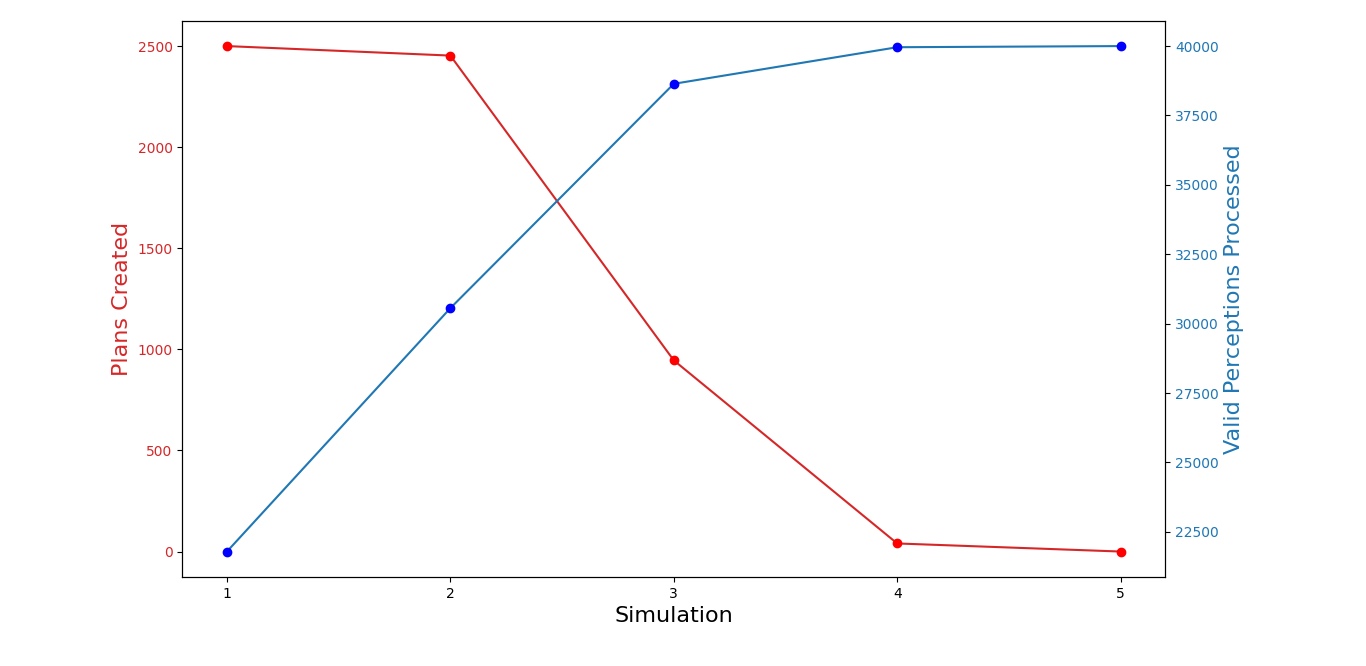
\includegraphics[width=\textwidth]{Images/perceptions_vs_plans.png}
    \caption{Evolução das percepções válidas processadas e dos planos novos criados ao longo das simulações}
    \label{fig:perceptions_v_plans-experiment3}
\end{figure}